\documentclass[11pt]{amsbook}
\usepackage[turkish]{babel}

\usepackage{../Ceyhun}
\usepackage{../amsTurkish}

\begin{document}

\begin{figure}[htb]
	\centering
	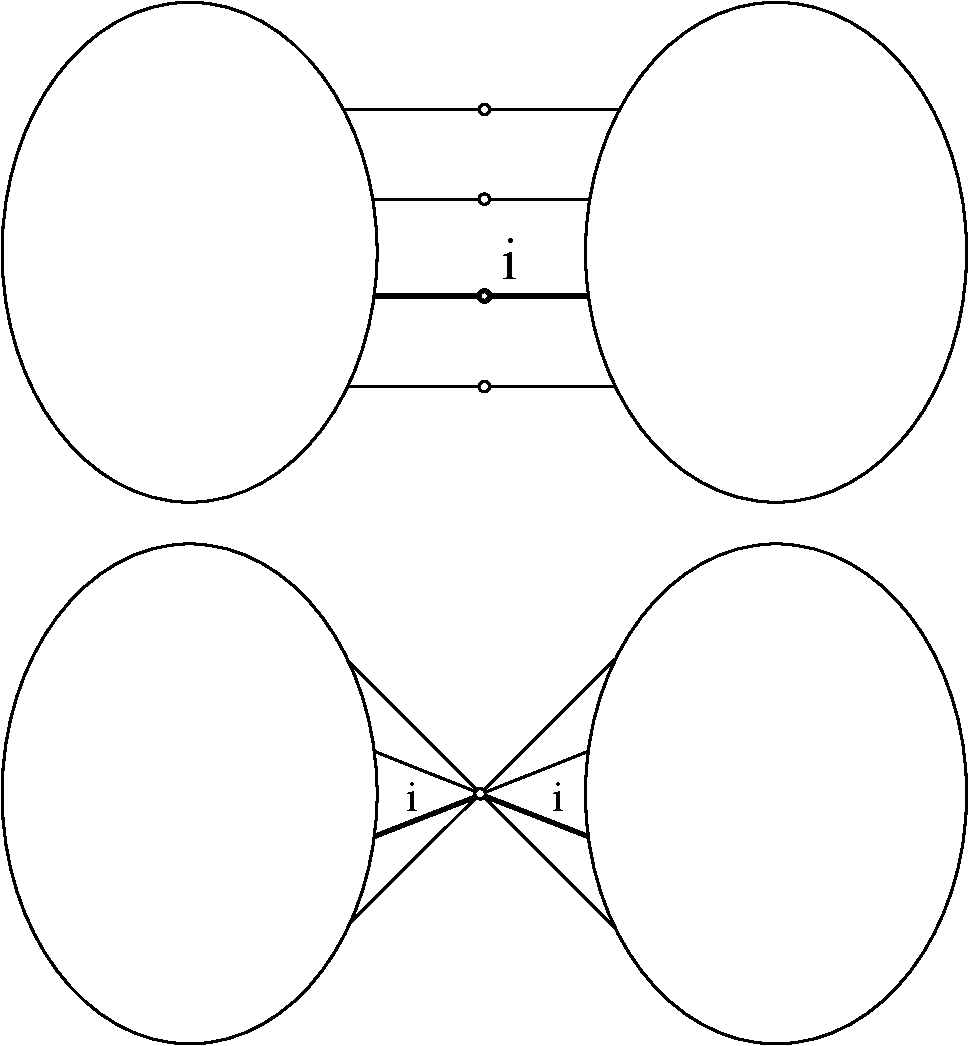
\includegraphics[width=0.4\textwidth]{images/ceyhun-047-fig01}
	\caption{\( M \)-matrisinin açıklanması}
	\label{fig:mMatrisininAciklanmasi}
\end{figure}

Bu çizgeleri, \reffig{fig:mMatrisininAciklanmasi}'de açıklandığı gibi, \( i \)
kesitlemesindeki ayrıtları büzüştürüp, çizgeyi ikiye ayırarak da elde
edebilirdik. \( Ç_1 \) ya da \( \bar{Ç}_2 \) çizgesinin t-kesitleme
matrisinin, \( Q_t \) matrisinden de elde edilebileceğini, aşağıdaki tanımı
verdikten sonra kolayca görebiliriz.

\begin{definition}
	\[
		{ M(i) }_1 = Q_t \ominus { H(i) }_2
	\]
	ve
	\[
		{ M(i) }_2 = Q_t \ominus { H(i) }_1
	\]

	olarak gösterilen ve \hDefined{\( M \)-matrisi} diye adlandıracağımız matrisler,
	\( Q_t \) matrisinden sırasıyla, \( { H(i) }_2 \) ve \( { H(i) }_1 \)
	matrisine ilişkin bütün dizek ve dikeçlerin atılması ile
\end{definition}

\end{document}
